% Method-of-lines workflow for Lecture 7.  The figure makes one directional
% modeling decision visible: discretize space first, then apply the DAE and
% collocation machinery already introduced in the lecture.
%
% GREYSCALE: the stages are labelled and connected by arrows; colour only
% reinforces the progression.  Base TikZ only.

\definecolor{cpblue}{HTML}{0072B2}
\definecolor{cporange}{HTML}{E69F00}

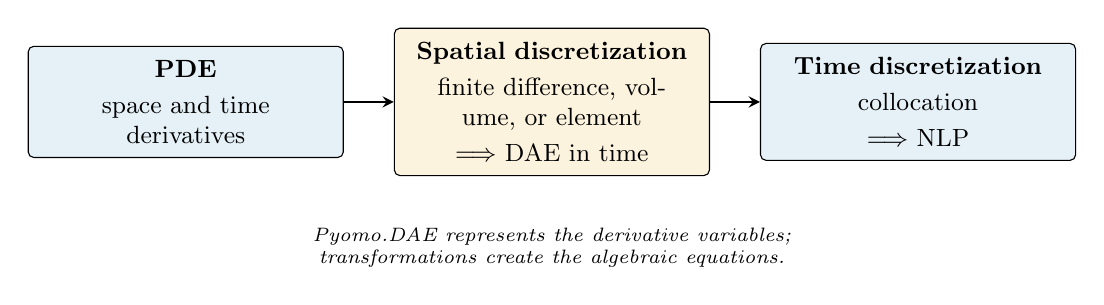
\begin{tikzpicture}[x=1cm, y=1cm, font=\small,
  stage/.style={draw, rounded corners=2pt, minimum height=1.35cm,
                text width=3.65cm, align=center, inner sep=5pt},
  flow/.style={->, >=stealth, thick}]
  \node[stage, fill=cpblue!10] (pde) at (0,0)
    {\textbf{PDE}\\[2pt] space and time derivatives};
  \node[stage, fill=cporange!13] (dae) at (4.65,0)
    {\textbf{Spatial discretization}\\[2pt] finite difference, volume, or element\\[2pt]
     $\Longrightarrow$ DAE in time};
  \node[stage, fill=cpblue!10] (nlp) at (9.3,0)
    {\textbf{Time discretization}\\[2pt] collocation\\[2pt]
     $\Longrightarrow$ NLP};
  \draw[flow] (pde) -- (dae);
  \draw[flow] (dae) -- (nlp);
  \node[align=center, font=\scriptsize\itshape] at (4.65,-1.85)
    {Pyomo.DAE represents the derivative variables;\\
     transformations create the algebraic equations.};
\end{tikzpicture}
